% Chapter 2

\chapter{Marco Teórico} % Main chapter title

\label{Chap:Marco} % For referencing the chapter elsewhere, use \ref{Chapter2} 

%----------------------------------------------------------------------------------------

% Define some commands to keep the formatting separated from the content 
%\newcommand{\keyword}[1]{\textbf{#1}}
%\newcommand{\tabhead}[1]{\textbf{#1}}
%\newcommand{\code}[1]{\texttt{#1}}
%\newcommand{\file}[1]{\texttt{\bfseries#1}}
%\newcommand{\option}[1]{\texttt{\itshape#1}}

%----------------------------------------------------------------------------------------

\section{El sistema de Posicionamiento Global - GPS}

\begin{figure}[ht]
\centering
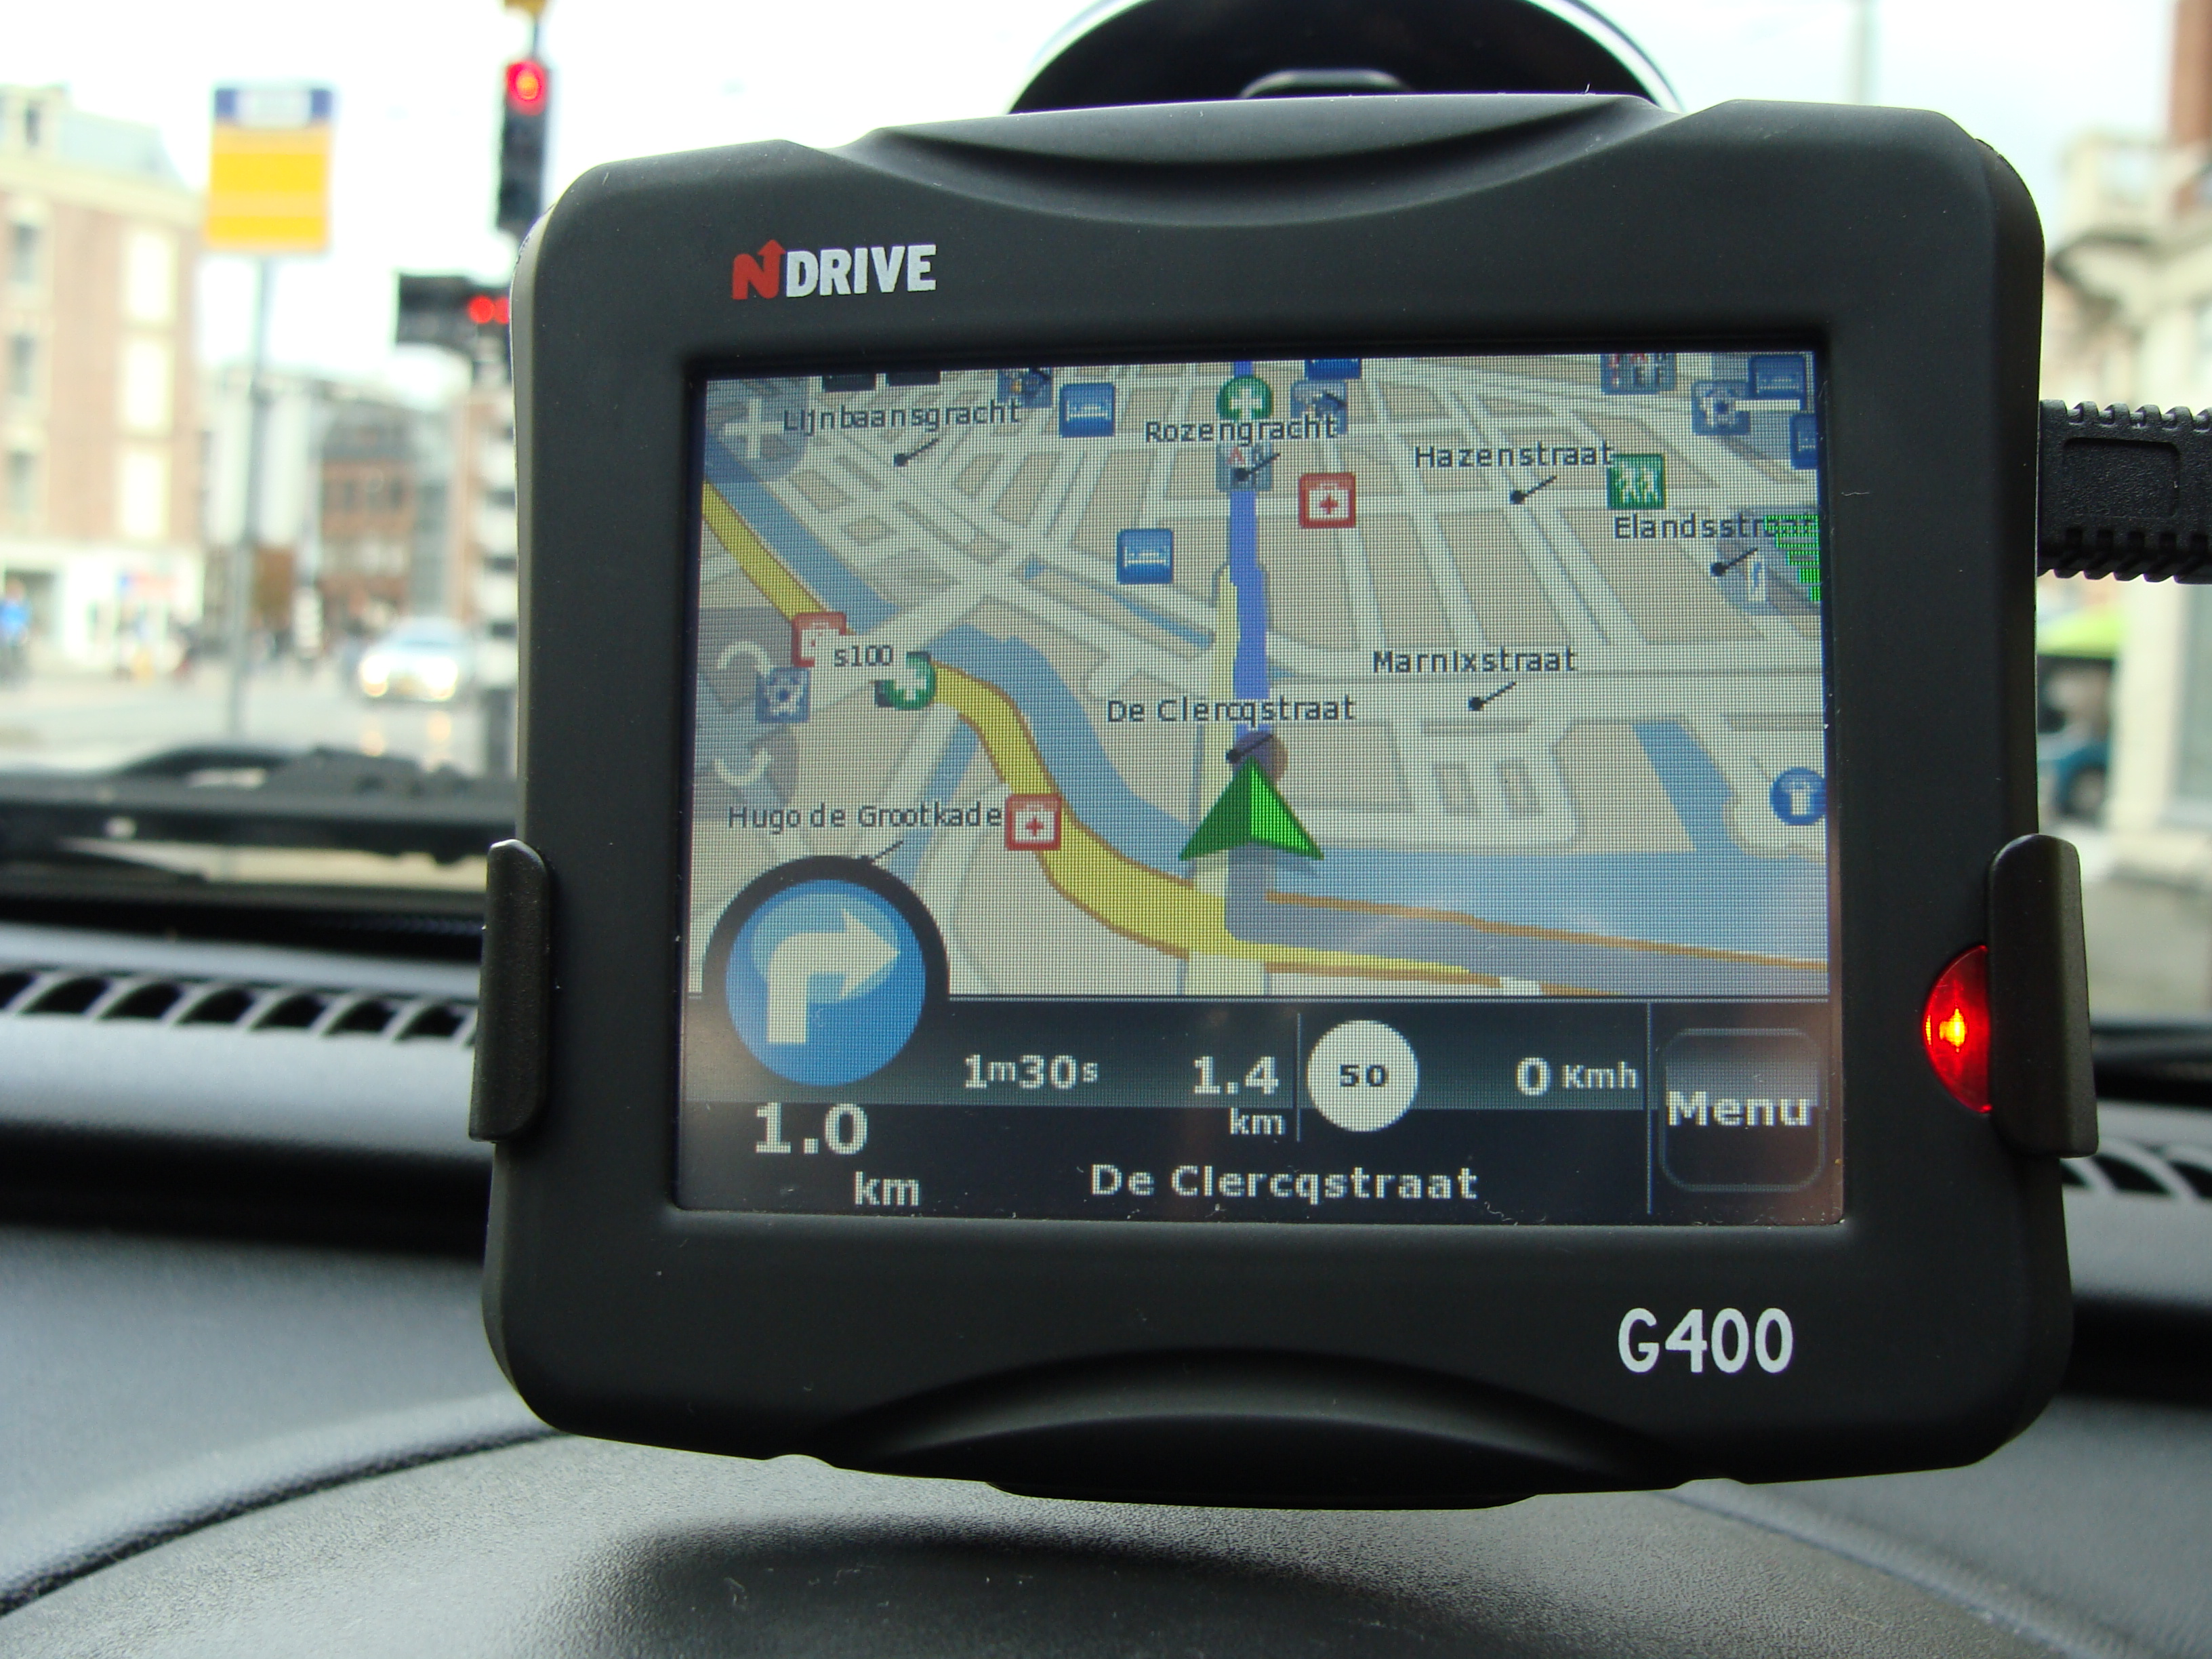
\includegraphics[scale=0.075]{Figures/GPS}
\caption[Sistema de Posicionamiento Global.]{Sistema de Posicionamiento Global.}
\label{fig:GPS}
\end{figure}

GPS fue iniciado en 1973 para su uso con fines militares por los Estados Unidos de Norteamérica. Su objetivo principal es la determinación de las coordenadas espaciales bajo una referencia mundial. Para dichos propósitos, se necesita una recepción de señales de un mínimo de cuatro satélites, cuyas coordenadas son plenamente conocidas
\textbf{[Huerta, E.; Mangiaterra, A.; Noguera, G. 2005]}.

\subsection{La constelación NAVSTAR}

\begin{figure}[ht]
\centering
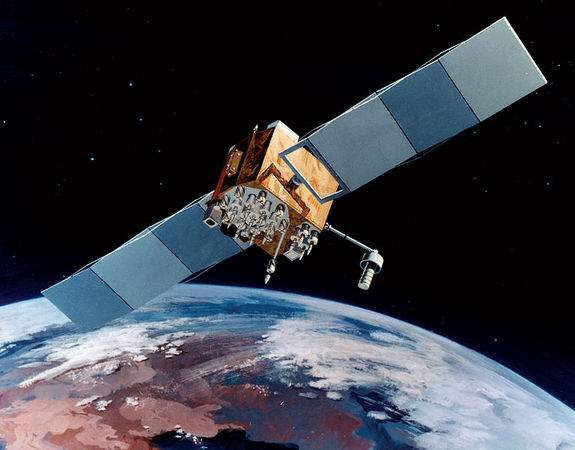
\includegraphics[scale=0.29]{Figures/Navstar}
\caption[Satélite de la constelación NAVSTAR.]{Satélite de la constelación NAVSTAR.}
\label{fig:NAV}
\end{figure}

La constelación NAVSTAR está conformada por los satélites que se utilizan para triangular la posición. Se propuso que fueran 24 satélites situados en seis planos de cuatro satélites cada uno con cobertura en toda la Tierra. \\

En 1983, el presidente Ronald Reagan permitió el uso civil del sistema, no sin antes añadir un error (llamado \textit{Disponibilidad Selectiva}) para evitar que fuese tan preciso. \\

En el año 2000, el presidente Bill Clinton retiró el error intencionado \textbf{[Zambrano Termal, Jhon. 2014]}.

\subsection{Dispositivos GPS}
Los dispositivos GPS son aparatos que obtienen la información de los satélites y realizan un procesamiento del mismo para ubicarse en el marco de referencia terrestre. \\

Existen GPS de distintos tamaños y marcas.

\begin{table}[!htb]
\begin{center}
\caption{Características del GPS Navspark RAW.}
\begin{tabular}{|l|}
	\hline
	        \ \ \ \ \ \ \ \ \ \ \ \ \ \ \ \ \ \ \ \ \ \ \ \ \ \ \ \ \ \ \ \ \ \ \ \ \ \ \ \ \ \ \ \ \ \ \ \ \ \ \textbf{Navspark RAW GPS} \\
	\hline
	%\begin{figure}[H]%Example image
		\\  \ \ \ \ \ \ \ \ \ \ \ \ \ \ \ \ \ \ \ \ \ \ \ \ \ \ \ \ \ \ \ \ \ \ \ \ \ \ \ \ 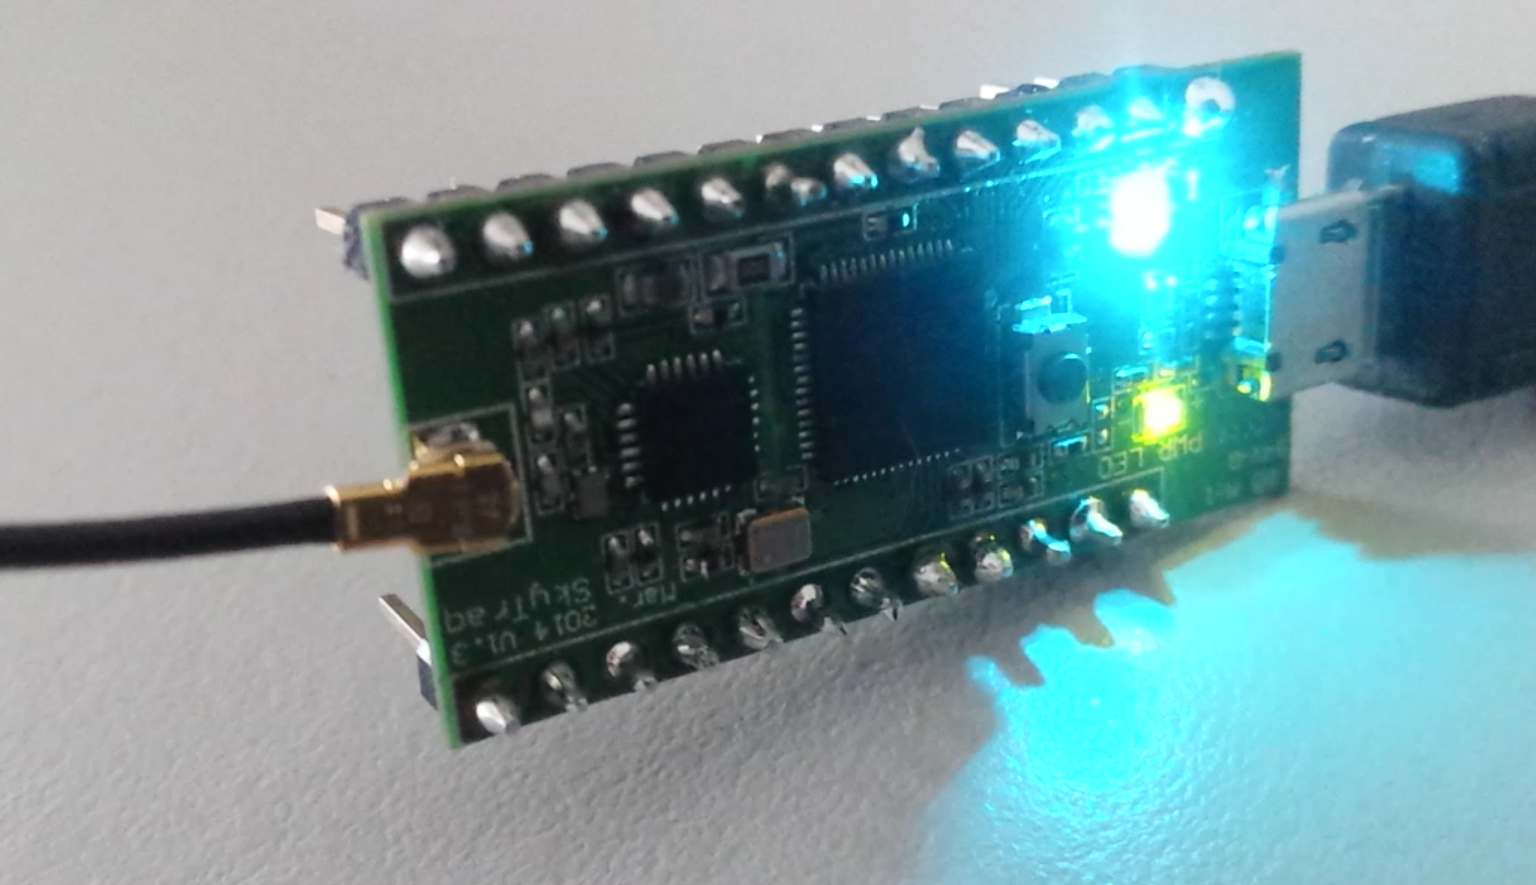
\includegraphics[width=0.37\linewidth]{Figures/NavGPS}
	%	\caption{GPS Navspark.}
		\label{fig:nsraw}\\
	%\end{figure} \\
	
	\textbf{Características:}\\
	%\begin{itemize}
		\tabitem Procesador: 100MHz 32bit LEON3 Sparc-V8 + IEEE-754 Compliant FPU.\\
		\tabitem 17 Digital I/O.\\
		\tabitem GPS con actualización de hasta 20 Hz.\\
		\tabitem Rango de operación: (h $<$ 18000 msnm) \& (v $<$ 515 m/s).\\
		\tabitem Precisión de hasta 2.5 metros.\\
		\tabitem Consumo: 15 ma @ 3.3V.\\
	%\end{itemize} \\
	\hline
\end{tabular}
\end{center}
\end{table}

\begin{table}[!htb]
\begin{center}
\caption{Características del GPS Ublox C94 M8P.}
\begin{tabular}{|l|}
	\hline
	\ \ \ \ \ \ \ \ \ \ \ \ \ \ \ \ \ \ \ \ \ \ \ \ \ \ \ \ \ \ \ \ \ \ \ \ \ \ \ \ \ \ \ \ \ \ \ \ \ \textbf{Ublox C94 M8P GPS}\\
	\hline
	%\begin{figure}[H] % Example image
	      \ \ \ \ \ \ \ \ \ \ \ \ \ \ \ \ \ \ \ \ \ \ \ \ \ \ \ \ \ \ \ \ \ \ \ \ \ \ \ \ 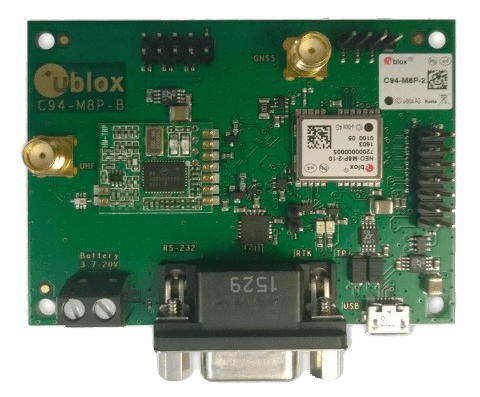
\includegraphics[width=0.37\linewidth]{Figures/ublox}\footnotemark
	%\caption{GPS Ublox. \footnotemark}
	\label{fig:ubx} \\
	%\end{figure} \\
	\textbf{Características: }\\

	%\begin{itemize}
		\tabitem 72 channel u-blox M8 engine GPS L1C/A, GLONASS L1OF, BeiDou B1.\\
		\tabitem GPS con actualizaciones de hasta 10 Hz.\\
		\tabitem Rango de operación: (h $<$ 50000 msnm) \& (v $<$ 500 m/s).\\
		\tabitem Precisión de hasta 2.5 metros.\\
		\tabitem Consumo: 23 ma @ 3.3V.\\
		\tabitem \textcolor{blue}{Incluye módulo de radiofrecuencia.}\\
	%\end{itemize} \\
	\hline
\end{tabular}
\end{center}
\end{table}

\footnotetext{Imagen alojada en www.u-blox.com}

\FloatBarrier

\newpage

\subsection{Fundamento matemático}

\subsection{Causas de error}

Como en todo sistema de medición, es probable que un cálculo de una posición se vea afectado por cualquiera de las siguientes: 

\begin{itemize}
	\item Satélites.
	\item Atmósfera.
	\item Rutas múltiples.
	\item Receptor.
\end{itemize} 

\subsubsection{Error causado por el satélite}

\begin{figure}[ht]
\centering
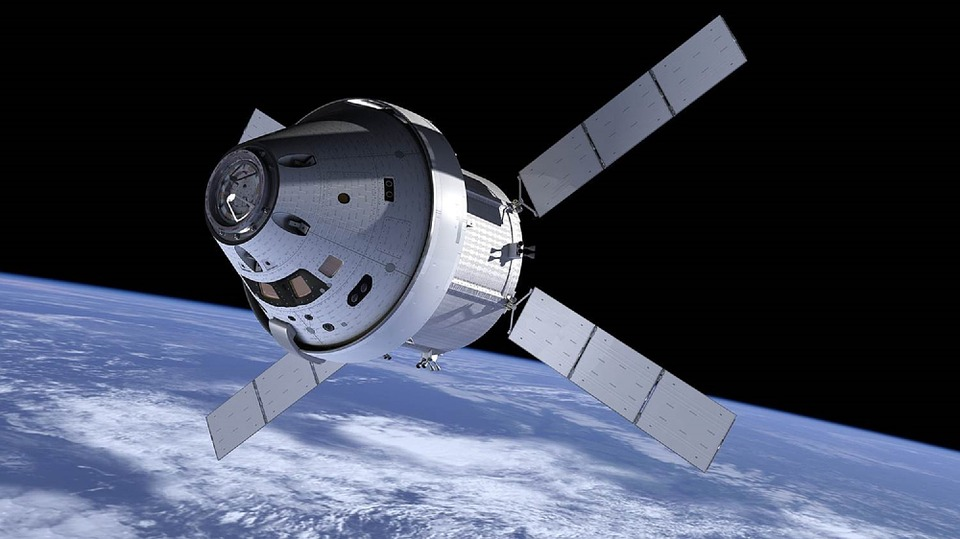
\includegraphics[scale=0.23]{Figures/Sat}
\caption[Error del reloj atómico satelital.]{Error del reloj atómico satelital.}
\label{fig:ErrSat}
\end{figure}

Los satélites incorporan relojes atómicos de gran exactitud. Como el tiempo es crítico al momento de la triangulación de cualquier dispositivo, un error de apenas un nanosegundo equivale a un error en distancia de 30 cm. Los relojes atómicos acumulan un error de esta magnitud cada tres años. \\

También, al error en la posición de los satélites sobre sus órbitas se le atribuye un error de 2.1 metros.

\subsubsection{Error causado por la atmósfera}

\begin{figure}[ht]
\centering
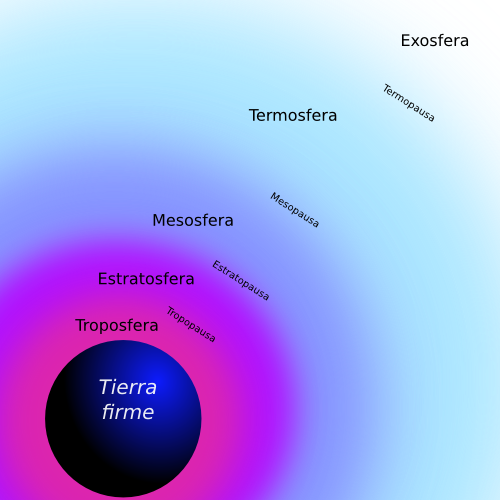
\includegraphics[scale=0.48]{Figures/CapasAtm}
\caption[Error por capas de la Atmósfera.]{Error por capas de la Atmósfera.}
\label{fig:ErrAtm}
\end{figure}

Las señales de radio que comunican a los satélites y los receptores deben atravesar a la atmósfera a través de considerables kilómetros. El sólo hecho de atravesar partículas cargadas en la ionósfera\footnotemark y entrar en contacto con el vapor de agua de la tropósfera causa variaciones de velocidad en la transmisión. \\

El error en distancia atribuible a esta etapa es de 4 metros. 

\footnotetext{El error obtenido en la ionósfera puede eliminarse utilizando receptores de frecuencia doble L1 y L2.}

\subsubsection{Error causado por rutas múltiples}

\begin{figure}[ht]
\centering
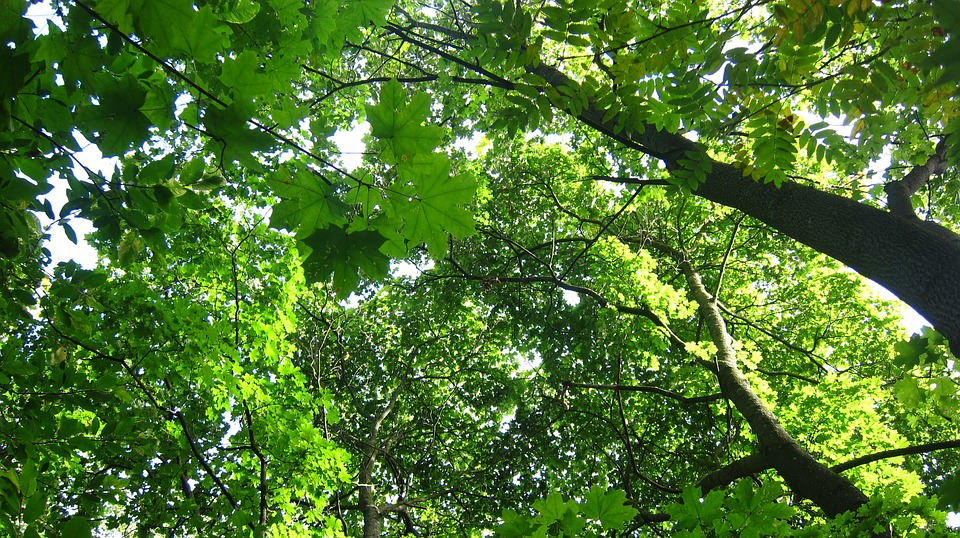
\includegraphics{Figures/RutasMult}
\caption[Error por rutas múltiples.]{Error por rutas múltiples.}
\label{fig:ErrRMul}
\end{figure}

 El sistema está diseñado para funcionar idealmente a cielo abierto. Sin embargo, en condiciones normales, esto no puede ser del todo reproducible, ya sea por el uso en áreas forestales o áreas urbanas. \\
 
Normalmente, la señal directa llega primero al receptor, y después, arriban las que proceden de las rutas múltiples. Esta diferencia de tiempo ocasiona otro error de medición. \\

Este mismo efecto era visible en las señales análogas de televisión, en las imágenes dobles. \\

Las nuevas antenas exteriores pueden filtrar este efecto.

\subsubsection{Error causado por el receptor}

Así como los satélites, los receptores cuentan con sus propios relojes. Debido a costos y dimensiones, éstos no pueden ser atómicos y por tanto son menos exactos, siendo otra fuente de error en la medición.\\

El error asociado a esta causa suele ser de 0.5 metros \textbf{[Fallas, 2002]}.

\subsubsection{Error por Disponibilidad Selectiva}

\begin{figure}[ht]
\centering

\includegraphics[scale=0.30]{Figures/RonaldReagan}
\caption[Error por Disponibilidad Selectiva.]{Error por Disponibilidad Selectiva.}
\label{fig:ErrDis}
\end{figure}

----- de Zambrano Thermal...

\section{Comunicación inalámbrica}

\begin{figure}[ht]
\centering
\includegraphics[scale=0.14]{Figures/Wireless}
\caption[Símbolo de conectividad inalámbrica.]{Símbolo de conectividad inalámbrica.}
\label{fig:ErrWrl}
\end{figure}

Se dice que dos dispositivos se comunican de forma \textbf{inalámbrica} cuando éstos interactúan sin un contacto sólido entre sus masas. \\

En los aparatos electrónicos, se suelen usar ondas de radiofrecuencia, que a su vez se subclasifican dependiendo de la frecuencia a la que son emitidas.\\

A menor frecuencia, se obtiene una gran cobertura pero la capacidad se ve mermada. Conforme se aumenta la frecuencia, se pierde capacidad de cobertura pero la carga que puede tener una banda, aumenta. Se dice entonces que es una relación inversamente proporcional.\\

Actualmente no existe algún organismo internacional que regule las frecuencias utilizadas...

\begin{table}[!htb]
\begin{center}
\caption{Bandas de frecuencia en comunicación inalámbrica.}
\begin{tabular}{|l|l|l|l|l|}
	\hline
	\textbf{País/Región} & \textbf{LF} & \textbf{HF} & \textbf{UHF} & \textbf{Microondas}\\
	\hline
	USA & 125-134 KHz & 13.56 MHz & 902-928 MHz & 2400-2483.5 MHz\\& & & & 5725-5850 MHz \\
	\hline
	Europa & 125-134 KHz & 13.56 MHz & 865-868 MHz & 2.45 GHz \\
	\hline
	Japón & 125-134 KHz & 13.56 MHz & No permitida & 2.45 GHz \\
	\hline
	China & 125-134 KHz & 13.56 MHz & No permitida & 2446-2454 MHz \\
	\hline
\end{tabular}
\end{center}
\end{table}

Continuar choro de Tapia, D. I., Cueli, J. R., García, Ó., Corchado, J. M., Bajo, J., \& Saavedra, A. (2007). Identificacion por radiofrecuencia: fundamentos y aplicaciones. Proceedings de las primeras Jornadas Científicas sobre RFID. Ciudad Real, Spain, 1-5.

\subsection{Protocolo ZigBee}

El estándar IEEE 802.15.4, mejor conocido como ZigBee, es una especificación para aplicaciones de control remoto para cualquier equipo que requiera de un bajo costo y un bajo consumo de potencia en entornos reducidos. ZigBee puede funcionar a tres bandas de frecuencia diferentes: 868 MHz, 915 MHz y 2.4 GHz. \\

\begin{figure}[ht]
\centering
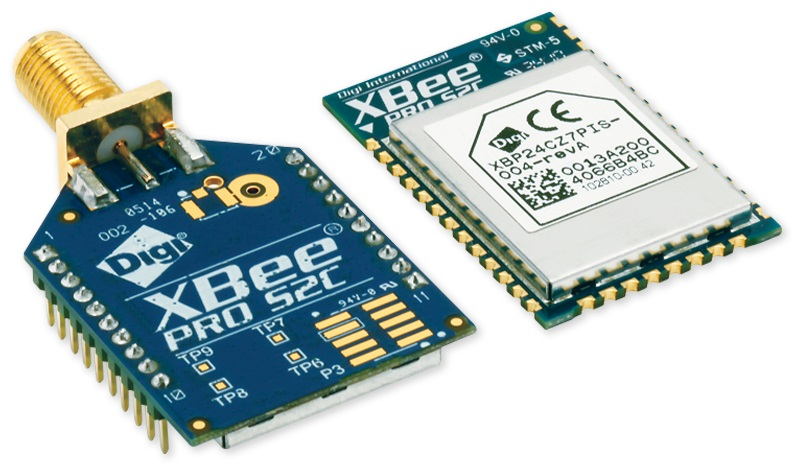
\includegraphics[scale=0.20]{Figures/xbee}
\caption[Equipo XBEE.]{Equipo XBEE.}
\label{fig:XBEE}
\end{figure}

Los módulos XBEE, fabricados por Digi International siguen el protocolo ZigBee. De entre todos esos módulos, destacan los de la serie PRO, ya que poseen una mayor potencia en la señal y en consecuencia, pueden hasta duplicar la capacidad de alcance en la distancia de transmisión. \\

El módulo requiere una alimentación que va desde los 2.8 V hasta los 3.4 V.

\subsection{Módulo UHF del Ublox C94-M8P GPS}

Los dispositivos GPS Ublox C94-M8P están diseñados para trabajar en pares y vienen incorporados con módulos de comunicación inalámbrica que operan en los 915 MHz de frecuencia en el continente americano. \\

En él, se puede configurar el envío y recepción de diferentes contenidos. El manual de Ublox recomienda usar el formato RTCM3, que será explicado más adelante.

\section{Sistemas de cómputo embebidos}

Los Sistemas Embebidos son sistemas programables, que realizan tareas específicas determinadas por el usuario, con el objetivo de optimizar los procesos para mejorar su desempeño y eficiencia, reduciendo tamaño y costos de producción. \\

Se caracterizan por el bajo consumo de energía. Está compuesto por tres componentes principales: Procesador, Dispositivos de almacenamiento y Periféricos [Caballero Paz, Andrés. 2014].

\subsection{BeagleBone Black}

\begin{figure}[ht]
\centering
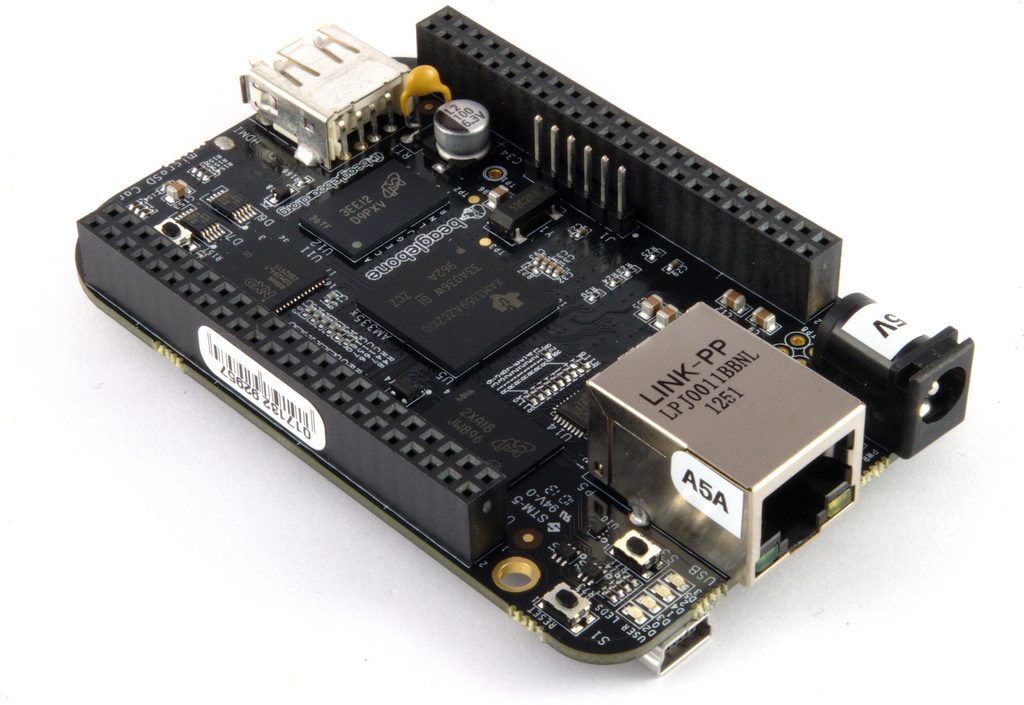
\includegraphics[scale=0.18]{Figures/BeagleBoneBlack}
\caption[BeagleBone Black.]{BeagleBone Black.}
\label{fig:ErrSat}
\end{figure}

La BeagleBone es una plataforma de desarrollo de bajo costo. \\

Desarrollada por la BeagleBone Foundation de los Estados Unidos, una fundación sin ánimos de lucro, cuyo objetivo es la promoción de hardware y software de código abierto para el desarrollo de sistemas embebidos. \\

Por su diseño, posee una arquitectura ARM, que posee soporte de varias distribuciones Linux [Coronado Vallés, Jorge. 2014]. \\

Por su condición de hardware y software abierto, tanto sus esquemáticos del hardware, como las códigos fuente de su software están disponibles a todos los usuarios. \\

De las ventajas que posee una arquitectura como la del BeagleBone, basada en microprocesadores, es que su uso conduce a plataformas más poderosas, capaces de realizar tareas de gran carga computacional [Coley, Gerald. 2013].

\section{Real Time Kinematics}

\begin{figure}[ht]
\centering
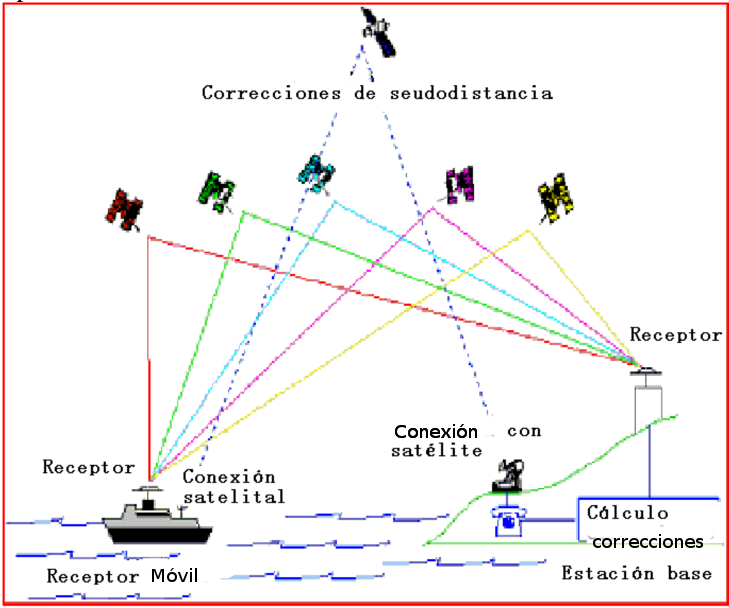
\includegraphics[scale=0.30]{Figures/DGPS1}
\caption[Esquema de funcionamiento en RTK.]{Esquema de funcionamiento en RTK.}
\label{fig:RTK}
\end{figure}

Se le llama Sistema de Navegación Cinética Satelital en Tiempo Real (RTK, Real Time Kinematics por sus siglas en inglés), a las correcciones de la señal del GPS basadas en las señales L1 y L2. \\

Todo está en torno al siguiente supuesto: \\

Se tienen dos receptores a una distancia de pocos km entre sí. En esta condición, se podría esperar que los errores causados por el reloj atómico del satélite, por la ionósfera y la tropósfera afectarían de igual manera y con la misma magnitud a ambos receptores, por su proximidad. Si la posición exacta de uno de los receptores es conocida, entonces esta información puede ser usada para determinar el error asociado a las lecturas de dicho receptor y después aplicar la corrección al otro dispositivo. \\

Al GPS cuya posición es conocida recibe el nombre de \textbf{receptor base} y el segundo es llamado \textbf{receptor móvil}. La estación base calcula la distancia entre cada uno de los satélites de los que recibe señal y su posición (también conocida) para determinar el error asociado a la medición de distancia. Esa información la envía al receptor móvil, quien aplica la corrección hacia dicho satélite, obteniendo así un conocimiento más exacto sobre su posición [Fallas, 2002]. \\

Con todas las correcciones aplicadas de forma ideal, se alcanza una precisión mejor a los 10 cm [Cerrato Miranda, Javier. 2011].

\section{Formato RTCM3}

Este formato es un estándar internacional para transmitir datos de posicionamiento en tiempo real. \\

El mensaje contendrá los siguientes datos: \\

\begin{table}[!htb]
\begin{center}
\caption{Contenido del mensaje en formato RTCM3.1}
\begin{tabular}{|l|}
	\hline
	\textbf{Mensaje RTCM3.1}\\
	\hline
	\tabitem \textbf{1005:} (X,Y,Z) Coordenadas fijas de la antena. \\
	\tabitem \textbf{1077:} Observaciones de GPS. \\
	\tabitem \textbf{1087:} Observaciones de GLONASS.\footnotemark \\
	\hline
\end{tabular}
\end{center}
\end{table}

\footnotetext{Homólogo ruso del sistema americano GPS.}

\section{RTKLIB}

Desarrollado por Tomoji Takasu, RTKLIB es un paquete de programas de código abierto para posicionamiento tanto estándar como preciso. Soporta varios modos de posicionamiento tales como: Simple, Diferencial, Cinemático, entre otros. \\

En todos sus modos soporta tanto procesamiento en tiempo real así como postprocesamiento.